% Results
\section{Results}
Three curves were chosen to demonstrate the aspects of the developed methods. The first is a family of curves, $Lissajous$ curves (\Cref{fig:lissajous}), which are a combination of two perpendicular harmonic oscillations. This curve was chosen due to the sharp changes in curvature and self-intersecting nature. The second curve, a tricuspoid (\Cref{fig:tricuspoid}) was chosen for the sharp, discontinuous features. In \Cref{fig:lissajous,fig:tricuspoid,fig:lastfigure} the curve is shown in red and the discretization is shown in black with vertices highlighted by circles indicating their position. Each curve was scaled so that the parameterization, $t$, was normalized between zero and unity. In each case the curve was originally discretized using one segment corresponding to a vertex located at $t=0$ and $t=1$. Once the original discretization is created, the discretizations are refined using \Cref{alg:discreteoptimize}. Further results can be found in \Cref{tab:curvelength}. In this table, the true lengths of the curves can be found. The combined length of the segments in each discretization are also given with the actual arc-length deficit.

\begin{figure}[h!]
  \centering
  \begin{tabular}{ccc}
  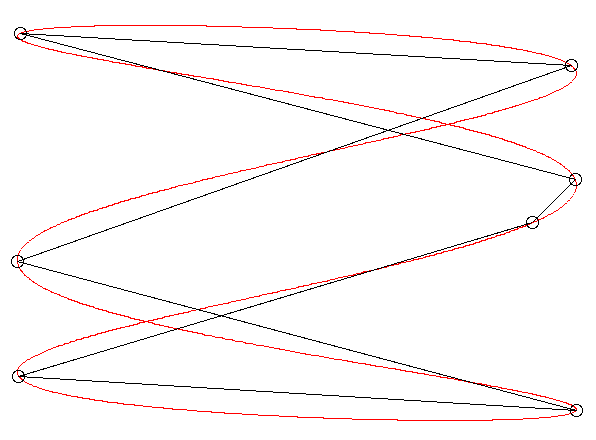
\includegraphics[width=0.3\linewidth]{Figures/lissajous01.png} &
  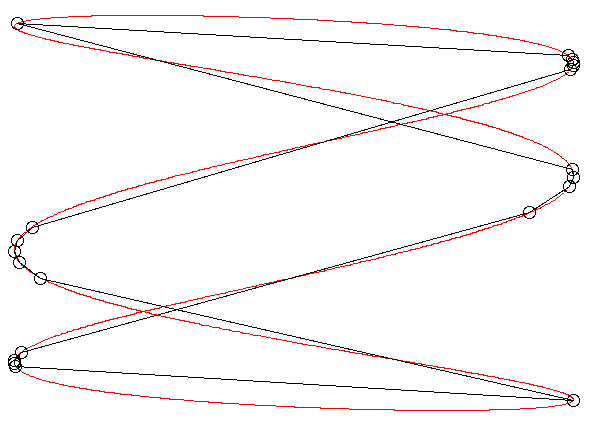
\includegraphics[width=0.3\linewidth]{Figures/lissajous001.png} &
  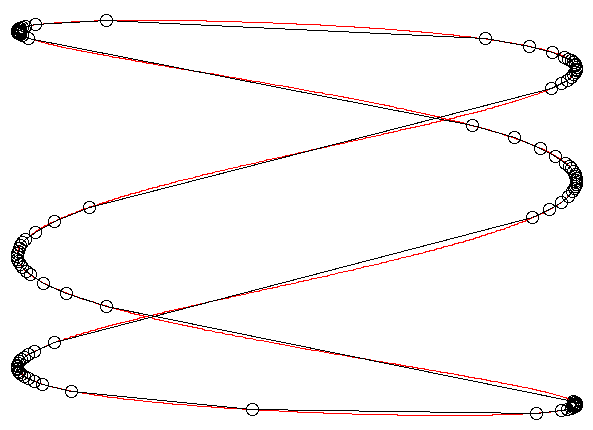
\includegraphics[width=0.3\linewidth]{Figures/lissajous0001.png}
  \end{tabular}
  \caption{\label{fig:lissajous} Lissajous Curves: 10\% deficit (left), 1\% deficit (middle), 0.1\% deficit (right)}
\end{figure}

For the Lissajous curve, the optimization can be seen to be effective and efficient with regards to only generating vertices where the curvature is high and not wasting vertices on the relatively ``straight'' portions of the curve. In addition, the self-intersection present on this curve did not impede the generation of an optimal edge-grid.

\begin{figure}[h!]
  \centering
  \begin{tabular}{ccc}
  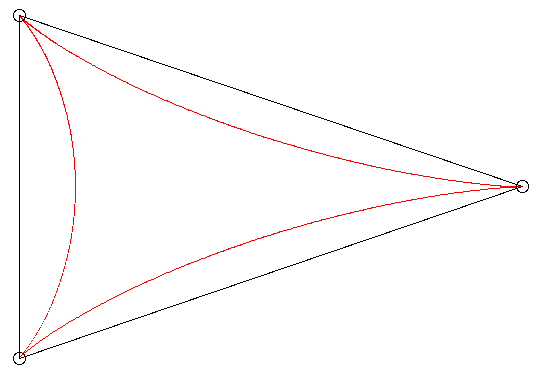
\includegraphics[width=0.3\linewidth]{Figures/tricuspoid01.png} &
  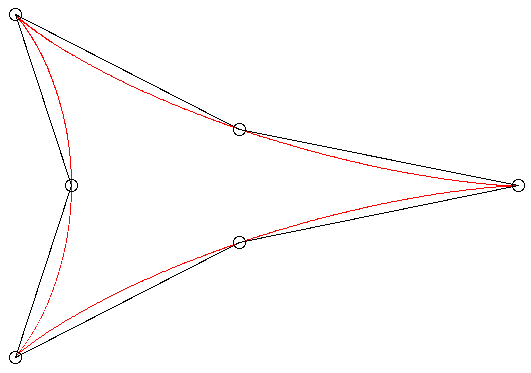
\includegraphics[width=0.3\linewidth]{Figures/tricuspoid001.png} &
  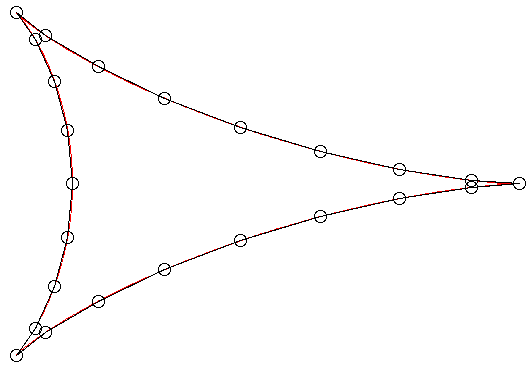
\includegraphics[width=0.3\linewidth]{Figures/tricuspoid0001.png}
  \end{tabular}
  \caption{\label{fig:tricuspoid} Tricuspoid Curve: 10\% deficit (left), 1\% deficit (middle), 0.1\% deficit (right)}
\end{figure}

For the Tricuspoid curve, the optimization can be seen to be accurate with regards to placing a vertex at the discontinuity. Placing a vertex at the discontinuity is efficient since not further nodes are required to capture that feature of the curve. It can be seen that further refinements are placed elsewhere on the curve.

\begin{figure}[h!]
  \centering
  \begin{tabular}{ccc}
  last & figure & here
  \end{tabular}
  \caption{\label{fig:lastfigure} Caption}
\end{figure}

\Cref{tab:curvelength} summarizes the results from discretizing the three curves. [REST OF PARAGRAPH ABOUT TABLE]

\begin{table}[h!] \caption{\label{tab:curvelength} Discretization length with respect to true curve length}
\begin{tabular}{cccc}
 & Lissajous Curve & Tricuspoid & last curve \\
True Length & 13.0653 & 16.0 & \\
10\% deficit criterion & 12.7123 (2.7\%) & 15.5885 (2.5\%) & \\
\end{tabular}
\end{table}
